% !TEX TS-program = pdflatex
% !TEX encoding = UTF-8 Unicode

\documentclass[11pt]{article}                                                   % use larger type; default would be 10pt
\usepackage[utf8]{inputenc}                                                     % set input encoding (not needed with XeLaTeX)

%%% PAGE DIMENSIONS ------------------------------------------------------------
\usepackage[top=0.8in, left=1in, right=1in, bottom=0.8in]{geometry}             % to change the page dimensions
\geometry{a4paper}                                                              % or letterpaper (US) or a5paper or....
\usepackage[parfill]{parskip}                                                   % Activate to begin paragraphs with an empty line rather than an indent

%%% HEADERS & FOOTERS ----------------------------------------------------------
\usepackage{fancyhdr}                                                           % This should be set AFTER setting up the page geometry
\pagestyle{fancy}                                                               % options: empty , plain , fancy
\renewcommand{\headrulewidth}{0pt}                                              % customise the layout...
\lhead{}\chead{}\rhead{}
\lfoot{}\cfoot{page \thepage}\rfoot{}

%%% SECTION TITLE APPEARANCE ---------------------------------------------------
\usepackage{sectsty}
\allsectionsfont{\sffamily\mdseries\upshape}                                    % (See the fntguide.pdf for font help)

%%% PACKAGES -------------------------------------------------------------------
\usepackage[font=small,labelfont=bf,textfont=it]{caption}                       % stylize captions
\usepackage{graphicx}                                                           % support the \includegraphics command and options
\usepackage{booktabs}                                                           % for much better looking tables
\usepackage{array}                                                              % for better arrays (eg matrices) in maths
\usepackage{paralist}                                                           % very flexible & customisable lists (eg. enumerate/itemize, etc.)
\usepackage{verbatim}                                                           % adds environment for commenting out blocks of text & for better verbatim
\usepackage{subfig}                                                             % make it possible to include more than one captioned figure/table in a single float
\usepackage{mathtools}                                                          % for math environments like align
\usepackage{amssymb}                                                            % for symbols like \therefore
\usepackage{verbatim}                                                           % for including text as appears, verbatim
\usepackage{listings}                                                           % for including external files as text, eg code
\usepackage{color}                                                              % for coloring of files and images
\usepackage{overpic}                                                            % for adding annotations to pictures
\usepackage{enumitem}
\usepackage{wrapfig}

%%% EQUATIONS ------------------------------------------------------------------
\numberwithin{equation}{section}                                                % Number equations by section (change for different levels)

%% BIBIOGRAPHY ------------------------------------------------------------------
\usepackage{cite}
\bibliographystyle{unsrt}

%%% ToC (table of contents) APPEARANCE -----------------------------------------
%\usepackage[nottoc,notlof,notlot]{tocbibind}                                   % Put the bibliography in the ToC
%\usepackage[titles,subfigure]{tocloft}                                         % Alter the style of the Table of Contents
%\renewcommand{\cftsecfont}{\rmfamily\mdseries\upshape}
%\renewcommand{\cftsecpagefont}{\rmfamily\mdseries\upshape}                     % No bold!

%%% PDF LINKS AND STYLE --------------------------------------------------------
\usepackage[unicode=true,
    bookmarks=true,bookmarksnumbered=true,bookmarksopen=true,
    bookmarksopenlevel=2, breaklinks=false,pdfborder={0 0 0},backref=false,
    colorlinks=false] {hyperref}                                                % for links in pdf file, no colors
\hypersetup{pdftitle={DOCUMENT NAME},
    pdfauthor={Josh Wainwright}}                                                % set name of document and author here

%%% END Article customizations

%%% Include TIKZ images directly into document ---------------------------------
\usepackage[svgnames]{xcolor}
\usepackage{tikz}
\usetikzlibrary{decorations.markings}
\usetikzlibrary{shapes.geometric}

\newif\iffinal                                                                  % introduce a switch for draft vs. final document
\finaltrue                                                                      % use this to compile the final document
\usepackage{tikz}

\iffinal
    \newcommand{\inputTikZ}[1]{%
        \input{#1}%
    }
\else
    \newcommand{\inputTikZ}[1]{%
        \beginpgfgraphicnamed{#1-external}%
        \input{#1}%
        \endpgfgraphicnamed%
    }
\fi

%%% Include svg images directly in document (requires Inkscape) ----------------
\newcommand{\executeiffilenewer}[3]{%
    \ifnum\pdfstrcmp{\pdffilemoddate{#1}}%
        {\pdffilemoddate{#2}}>0%
        {\immediate\write18{#3}}
    \fi
}
\newcommand{\includesvg}[1]{%
    \executeiffilenewer{#1.svg}{#1.pdf}%
    {inkscape -z -D --file=#1.svg --export-pdf=#1.pdf --export-latex}%
    \input{#1.pdf_tex}%
}

%%% NEW COMMANDS ---------------------------------------------------------------
\renewcommand{\d}{\,\mathrm{d}}                                                 % for integrals
\newcommand{\dx}[2]{\frac{\textrm{d} #1}{\textrm{d} #2}}                        % for derivatives
\newcommand{\dd}[2]{\frac{\textrm{d}^2 #1}{\textrm{d} #2^2}}                    % for double derivatives
\newcommand{\pd}[2]{\frac{\partial #1}{\partial #2}}                            % for partial derivatives
\newcommand{\pdd}[2]{\frac{\partial^2 #1}{\partial #2^2}}                       % for double partial derivatives
\newcommand{\e}[1]{\text{e}^{#1}}                                               % for exponentials
\newcommand{\code}[1]{\texttt{#1}}                                              % for verbatim code view
\newcommand{\inter}[1]{\shortintertext{#1}}                                     % shorter version of intertext
\newcommand{\under}[1]{\underline{#1}}                                          % for vectors etc.

\let\vaccent=\v                                                                 % rename builtin command \v{} to \vaccent{}
\newcommand{\uv}[1]{\ensuremath{\hat{#1}}}                                      % for unit vector
\newcommand{\abs}[1]{\left| #1 \right|}                                         % for absolute value
\newcommand{\avg}[1]{\left< #1 \right>}                                         % for average
\let\underdot=\d                                                                % rename builtin command \d{} to \underdot{}
\newcommand{\ket}[1]{\left| #1 \right>}                                         % for Dirac bras
\newcommand{\bra}[1]{\left< #1 \right|}                                         % for Dirac kets
\newcommand{\braket}[2]{\left< #1 \vphantom{#2} \right|
    \left. #2 \vphantom{#1} \right>}                                            % for Dirac brackets
\newcommand{\matrixel}[3]{\left< #1 \vphantom{#2#3} \right|
    #2 \left| #3 \vphantom{#1#2} \right>}                                       % for Dirac matrix elements
\newcommand{\grad}[1]{\nabla #1}                                                % for gradient
\let\divsymb=\div                                                               % rename builtin command \div to \divsymb
\renewcommand{\div}[1]{\nabla \cdot #1}                                         % for divergence
\newcommand{\curl}[1]{\nabla \times #1}                                         % for curl
\let\baraccent=\=                                                               % rename builtin command \= to \baraccent
\renewcommand{\=}[1]{\stackrel{#1}{=}}                                          % for putting numbers above =


%*******************************************************************************
%******************************** END HEADER ***********************************
%*******************************************************************************

\begin{document}
%!TEX root = Problems2_main.tex

\makeatletter
\renewcommand{\@maketitle}{
\newpage
 \null
 \vskip 2em%
 \begin{center}%
  {\Large \@title \par}%
 \end{center}%
 \par} \makeatother

\begin{center}
\Huge University Physics Problems 2\\[1em]
\large March 2013
\end{center}

\section{Reflecting}
	Two periscopes are constructed as shown below. In each case, the periscope is used to observe a person with the word BEN written on their t-shirt. In each case, the light is reflected from mirror 1 to mirror 2 and then to the observer. For each design, what is the orientation of the word as viewed by the observer?
	\begin{figure}[ht]
	  \centering
	  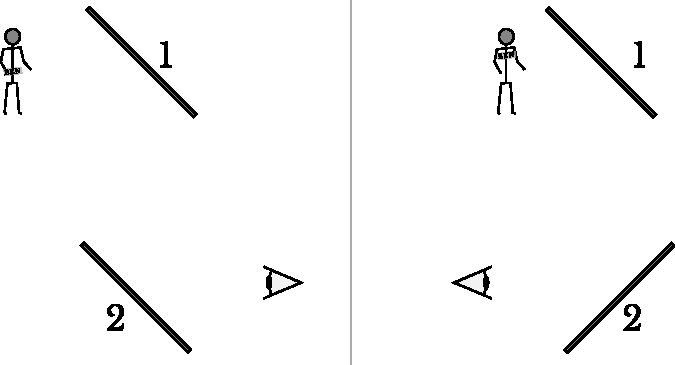
\includegraphics[width=0.6\textwidth]{periscopes.pdf}
	\end{figure}

\section{Recombining}
	A narrow beam of white light passes through a glass prism. The light is dispersed into its constituent colours. Can these rays be recombined into white light by passing them through a second prism?

\section{Throwing}
	\subsection{}
		\begin{wrapfigure}{r}{0.4\textwidth}
		  \vspace{-20pt}
		  \begin{center}
		  	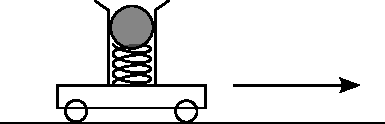
\includegraphics[width=0.35\textwidth]{trolley1.pdf}
		  \end{center}
		  \vspace{-20pt}
		\end{wrapfigure}
		A trolley rolls without friction along a track. When the trolley passes over some point in the track, the ball is released and is ejected upwards. Does it fall 
		\begin{enumerate}[label=\alph*)]
			\item infront of the tube,
			\item behind the trube,
			\item back into the tube?
		\end{enumerate}

	\subsection{}
		\begin{wrapfigure}{r}{0.4\textwidth}
		  \vspace{-20pt}
		  \begin{center}
		  	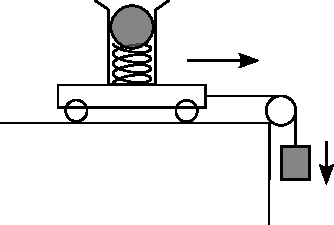
\includegraphics[width=0.35\textwidth]{trolley2.pdf}
		  \end{center}
		  \vspace{-20pt}
		\end{wrapfigure}
		The trolley is now connected via a light string and a pulley whell to a weight and the experiement repeated. Does the ball fall
		\begin{enumerate}[label=\alph*)]
			\item infront of the tube,
			\item behind the trube,
			\item back into the tube?
		\end{enumerate}

	\subsection{}
		\begin{wrapfigure}{r}{0.4\textwidth}
		  \vspace{-20pt}
		  \begin{center}
		  	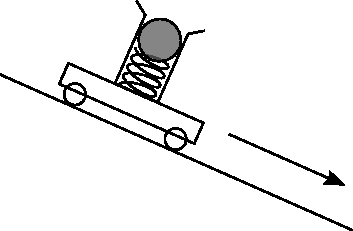
\includegraphics[width=0.35\textwidth]{trolley3.pdf}
		  \end{center}
		  \vspace{-20pt}
		\end{wrapfigure}
		The trolley is now connected via a light string and a pulley whell to a weight and the experiement repeated. Does the ball fall
		\begin{enumerate}[label=\alph*)]
			\item infront of the tube,
			\item behind the trube,
			\item back into the tube?
		\end{enumerate}


\clearpage
%!TEX root = Problems2_main.tex

% Remove the author and date fields and the space associated with them
% from the definition of maketitle!
\makeatletter
\renewcommand{\@maketitle}{
\newpage
 \null
 \vskip 2em%
 \begin{center}%
  {\Large \@title \par}%
 \end{center}%
 \par} \makeatother

\begin{center}
\Huge University Physcis Answers 1\\[1em]
\large March 2013
\end{center}
\setcounter{section}{0}

\section{Reflecting} % (fold)
	\label{sec:reflecting_ans}
	In the first case, the word will be the same as the original, in the second it will be inverted.

	The mirrors in each case invert the image. When orientated as in the first case, the combined reflections reverse the effect, in the second, the overall image is inverted.
	\begin{figure}[ht]
		\centering
		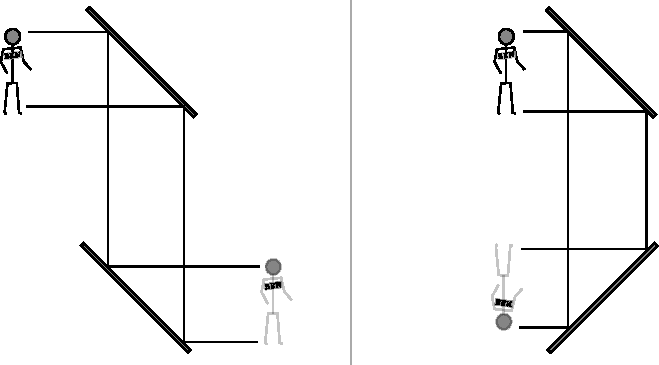
\includegraphics[width=0.5\textwidth]{periscopes_answers.pdf}
	\end{figure}
% section reflecting (end)

\section{Recombining} % (fold)
	\label{sec:recombining_ans}

	Yes.

	The light is dispersed into the rainbow since each wavelength travels at a slightly different speed through the glass. This implies that the wavelengths have different reflective indices in the glass and so are diffracted by slightly different amounts. As such when the light leaves the prism, the wavelengths have been separated out into the rainbow pattern. Thus, to recreate the original white light, the wavelengths simply need to be diffracted by the same amount in the opposite direction. This can be done using an exact copy of the first prism upside down relative to it.
% section recombining (end)

\section{Throwing} % (fold)
	\label{sec:throwing_ans}

	\subsection{c.} % (fold)
		\label{sub:1}
		The ball and the trolley move without friction, therefore, there are no forces acting upon them in the horizontal direction and so they will continue to move at constant velocity. Since any object travelling under only gravity will also maintain a constant horizontal velocity, the ball must move at the same speed along the track as the trolley, weather it is in the air or not. So it must land back in the tube.
	% subsection  (end)
	\subsection{b.} % (fold)
		\label{sub:2}
		The trolley is now subject to a constant force, and so will undergo constant acceleration. The ball, once ejected from the tube, does not feel the force and so travels at a constant velocity. Since, by the time it has flown up and then down it has maintained a constant velocity, but that the trolley has been accelerating, it must have travelled a shorter distance. Therefore it will land behind the trolley.
	% subsection  (end)
	\subsection{} % (fold)
		\label{sub:3}
		
	% subsection  (end)
% section throwing (end)

\section{Rolling} % (fold)
	\label{sec:rolling_ans}
	The drum moves right.

	In the first case, the drum rolls to the right since the string pulls the centre, causing the string to unwrap. In the second case, however, if the string unwraps, then the drum will move to the left. This can be discounted by considering the forces acting on the drum. There is a single force acting to the right, and no force to the left. Therefore, the drum cannot move left.

	Consider the torque on the drum taken about the base, where it touches the ground. There is a static friction force acting in the opposite direction to the force on the string, and then a torque caused by the string which makes the drum move to the right. This situation is the same as an upright block being pulled from the top, the block will topple in the direction it is pulled. In the case of the drum, it ``topples'', but this causes it to roll.

	\begin{figure}[ht]
		\centering
		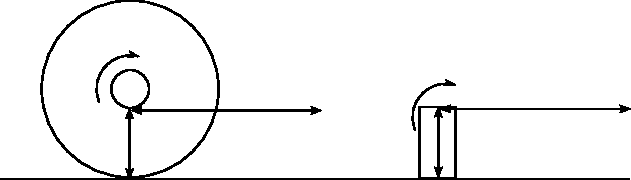
\includegraphics[width=0.5\textwidth]{drums_rolling_answer.pdf}
	\end{figure}
% section rolling (end)

\section{Illuminating} % (fold)
	\label{sec:illuminating_ans}
	After the first polaroid, the intensity of the light decreases as only one orientation of the light is allowed to pass through.

	After the two polaroids at ninety degrees, the intensity of the light is reduced to zero as the polarised light from the first polaroid is opposite to that which would pass through the second.

	When there are three polaroids, the intensity after all three increases compared to two above. The first allows only vertically polarised light though. The second allows some of the vertically polarised light through, but causes it to have a component in the horizontal direction. The third only allows horizontally polarised light through, but since the second cause some of the light to become polarised in this direction, some can get through the final polaroid. This means that the final intensity is now not zero.

	This principle is used in liquid crystal displays where molecules are used instead of the middle polaroid. If they are aligned, then the polaroids at either side let no light pass through them. But an electric field causes the molecules to line up so that they rotate the polarisation so it can get through the final barrier.
% section illuminating (end)

\end{document}

